\documentclass{article}
\usepackage[cmex10]{amsmath}
\usepackage{mathtools}
%\usepackage{txfonts}
\usepackage{wasysym}
\usepackage{amsthm}
\usepackage{mathrsfs}
\usepackage{table-fct}
%\usepackage{cite}
\usepackage{cases}
\usepackage{longtable}
\usepackage{enumerate}
\usepackage{enumitem}
%\usepackage[nottoc]{tocbibind}
%\usepackage[square,numbers]{natbib}
\usepackage{arxiv}
\usepackage{graphicx}
\usepackage[utf8]{inputenc} % allow utf-8 input
\usepackage[T1]{fontenc}    % use 8-bit T1 fonts
\usepackage{hyperref}       % hyperlinks
\usepackage{url}            % simple URL typesetting
\usepackage{booktabs}       % professional-quality tables
\usepackage{amsfonts}       % blackboard math symbols
\usepackage{nicefrac}       % compact symbols for 1/2, etc.
\usepackage{microtype}      % microtypography
\usepackage{lipsum}
\usepackage{subfig}
\usepackage{caption}
\usepackage{csquotes}
\usepackage{listings}
\usepackage{datetime}
\newcommand{\pasa}{PASA}
\newcommand{\jcap}{Journal of Cosmology and Astroparticle Physics}
\newcommand{\mnras}{Monthly Notices of the Royal Astronomical Society}
\newcommand{\aap}{Astronomy and Astrophysics}
\newcommand{\apjl}{Astrophysics Journal Letters}
\newcommand{\ptrsl}{Philosophical Transactions of Royal Society}

\usepackage[square,numbers]{natbib}
\captionsetup[figure]{labelfont=it,textfont={it}}
%\captionsetup[subfigure]{textfont=normalfont,singlelinecheck=off,justification=center}
\renewcommand{\bibsection}{\section*{\Large REFERENCES}}


%\bibliography{biblio.bib}
%\bibliography{ref}
\begin{document}
	\newcolumntype{P}[1]{>{\centering\arraybackslash}p{#1}}
	\title{Ice-Cube Data Analysis\\ \textit{B.Tech. Project - Fall 2022}}
	\Large
	\author{\huge
		Vibhavasu Pasumarti \\\\
		\Large
		EP20BTECH11015\\
		\Large
		Engineering Physics\\
		\Large
		Indian Institute of Technology, Hyderabad \\[1in]
		%\vspace{1in}
		\huge
		\textbf{Supervisor}\\\\
		\huge
		Dr. Shantanu Desai\\\\
		\Large
		Department of Physics\\
		\Large
		Indian Institute of Technology, Hyderabad 
	}
	\date{\today}	
\begin{center}
	
\includegraphics[width=0.75\textwidth]{Images/horzlogolong.png}
\end{center}
\maketitle 
\newpage
%\large
\tableofcontents
\newpage




\begin{abstract}
\large
%\section{OBJECTIVE}
The objective of this project was to determine angular correlation between radio pulsars and ultra-high energy neutrinos using the publicly available IceCube point source neutrino events catalog. For this purpose we use the
unbinned maximum likelihood method to search for a statistically significant excess from each of the pulsars in the ATNF catalog.
\end{abstract}
\newpage
\large
\section{\Large INTRODUCTION}
%\section{\large INTRODUCTION}
\subsection{\large Pulsars}
Pulsars are rapidly spinning neutron stars, which emit pulsed radio emissions with periods ranging from  milliseconds to a few seconds  with  magnetic fields ranging from $10^8$ to $10^{14}$ G. They are formed when massive rotating stars ($M \approx 12 - 15 M_\odot$) undergo supernovae leaving behind a small, dense core($M \approx 2 - 3.4 M_\odot$) supported by neutron degeneracy pressure. The collapsed core (comprised entirely of neutrons, hence, neutron star) retains most of the progenitor's angular momentum, while their moment of inertia is reduced sharply increasing their angular velocity.
\subsection{\large Neutrinos}
Neutrinos are fermionic particles that interact only via \underline{weak interactions and gravity}.
They are electrically neutral and have negligible rest mass.\\
Neutrinos are created by various radioactive decays, some of those  processes which are observed often are:
\begin{enumerate}
    \item Beta decay of atomic nuclei or hadrons
    \item Natural nuclear reactions (such as those that take place in the core of a star)
    \item Artificial nuclear reactions in nuclear reactors, nuclear bombs, or particle accelerators
    \item During a supernova
    \item During the spin-down of a neutron star
    \item When cosmic rays or accelerated particle beams strike atoms
\end{enumerate}
Neutrinos come in 3 \emph{flavours}:
\begin{enumerate}
    \item $e^- $
    \item $\mu$-on
    \item $\tau$
\end{enumerate}
reference https://en.wikipedia.org/wiki/Neutrino

\subsection{\large Neutrino detection methods}
Due to their negligible rest mass, the gravitational forces exerted by neutrinos cannot be used as a way to detect them. So they are detected with their interactions with matter.\\
Neutrinos interact with matter in two ways
\begin{enumerate}
    \item Neutral current interaction:\\
    \quad In a neutral current interaction, the neutrino enters and transferres some of its energy and momentum to a ‘target’ particle, and leaves the detector. If the target particle is charged and sufficiently lightweight, it might be accelerated to a relativistic speed and consequently emit Cherenkov radiation, which can be observed directly.\\
    However, this detection does not enable us to determine the \emph{flavour} of the neutrino
    \item Charged current interaction\\
    \quad In a charged current interaction, a high-energy neutrino transforms into its partner lepton ($e^-, \mu$, or $\tau$). However, if the neutrino does not have sufficient energy to create its heavier partner's mass, it cannot undergo a charged current interaction.
\end{enumerate}
%\newpage
\subsection{\large IceCube}
%ref:\url{https://icecube.wisc.edu/science/icecube/}
\\
%ref:\url{https://en.wikipedia.org/wiki/IceCube_Neutrino_Observatory}\\
The IceCube is a neutrino observatory constructed at the Amundsen–Scott South Pole Station in Antarctica.

\begin{figure}[htbp] % H here makes the images come at the correct position
	\centering
	\begin{minipage}{.5\textwidth}
		\centering
		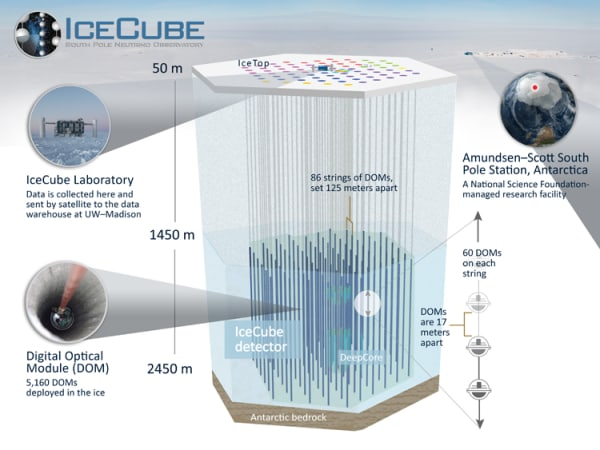
\includegraphics[width=0.8\linewidth]{Images/icecube_detector_schematic.jpg}
		\captionof{figure}{}
	\end{minipage}%
	\begin{minipage}{.5\textwidth}
		\centering
		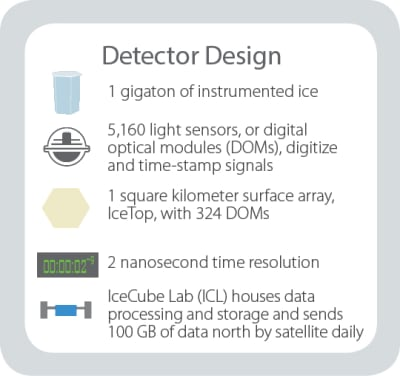
\includegraphics[width=0.65\linewidth]{Images/icecube_detector_design.jpg}
		\captionof{figure}{}
	\end{minipage}
	\caption*{Structure of IceCube Observatory}
\end{figure}
The %in-ice component of 
IceCube consists of 5,160 digital optical modules (DOMs), each with a ten-inch photomultiplier tube and associated electronics. The DOMs are attached to vertical “strings,” frozen into 86 boreholes, and arrayed over a cubic kilometer from 1,450 meters to 2,450 meters depth. The strings are deployed on a hexagonal grid with 125 meters spacing and hold 60 DOMs each. The vertical separation of the DOMs is 17 meters.

\subsection{\large Working principle}
The IceCube detects neutrinos via the Neutral current interactions. 
When they happen to interact with the ice they produce electrically charged leptons that in turn emit Cherenkov light, as a result of traveling through the ice faster than light travels in ice.

The IceCube sensors collect this light, which is subsequently digitized and time stamped. This information is sent to computers in the IceCube Lab on the surface, which converts the messages from individual DOMs into light patterns that reveal the direction and energy of muons and neutrinos.

When neutrinos (rarely) collide with the molecules of ice, they create charged leptons ($e^-$ $\mu$ons and $\tau$). If the created leptons are energetic enough, they emit Cherenkov radiation which is detected by photomultiplier tubes within the DOMs making up IceCube.

\begin{figure}[htb]
    \centering
    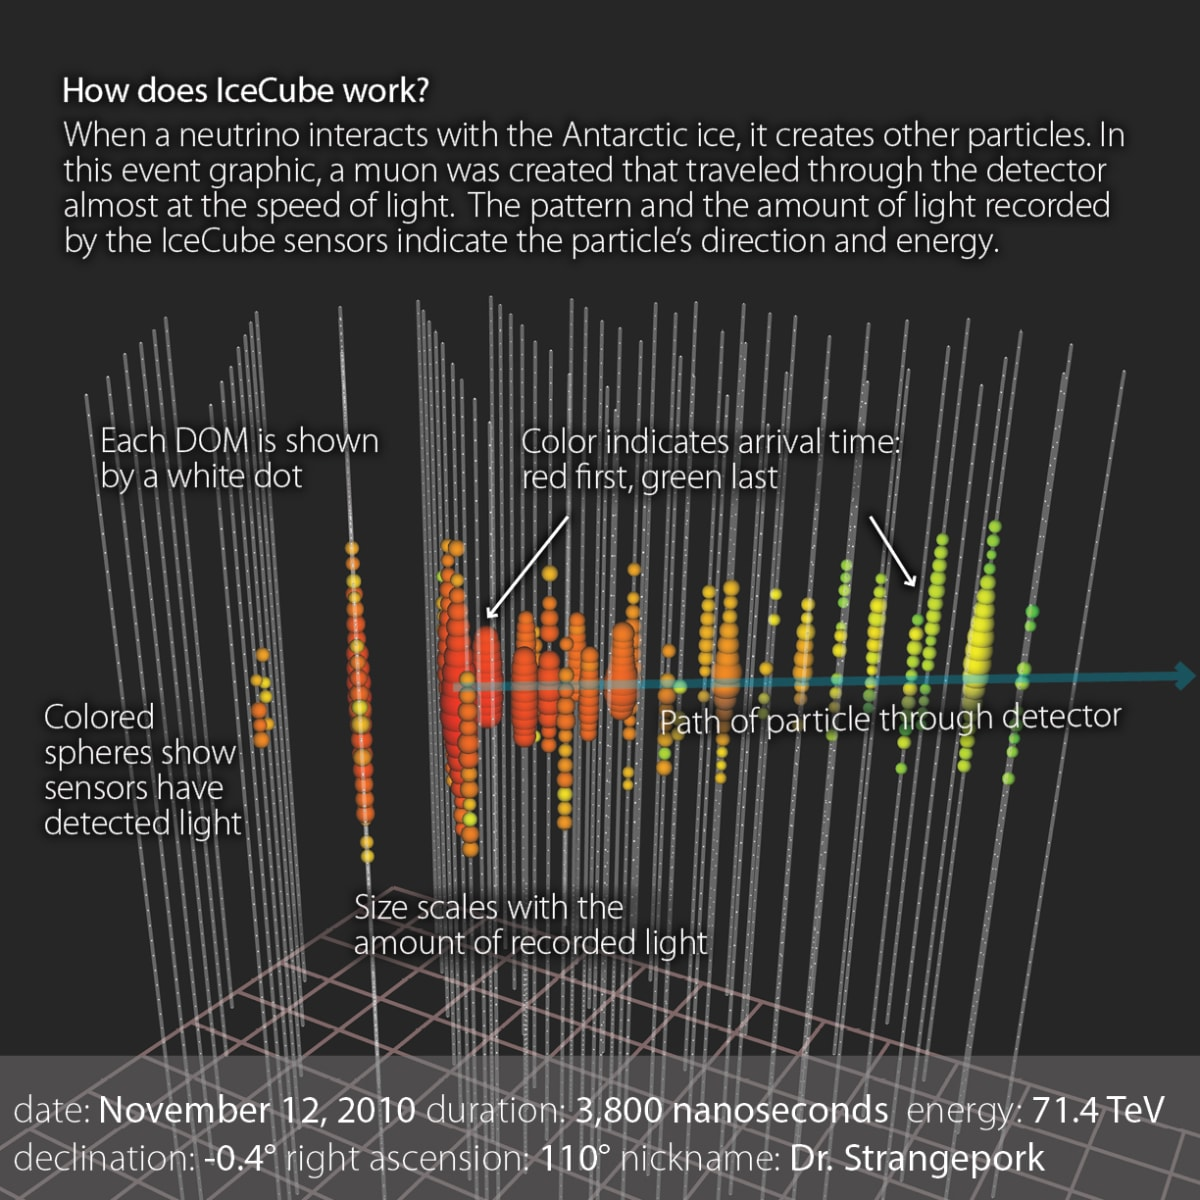
\includegraphics[width=0.5\textwidth,keepaspectratio]{Images/how_does_icecube_work.jpg}
    \caption{Structure of IceCube Observatory}
    \label{fig:IC_schematic}
\end{figure}
The IceCube is more sensitive to muons due to their greater penetration and longer detector tracks than other particles. An electron produced by an electron neutrino event to point back to sources because it scatters multiple times and loses energy below the Cherenkov threshold.




The IceCube is more sensitive to muons than others as they are the most penetrating and have the longest tracks in the detector. An electron resulting from an electron neutrino event scatters several times and loses enough energy to fall below the Cherenkov threshold, so they cannot be used to point back to sources. Tau leptons create short-lived cascade events which cannot travel very far before decaying, and are usually indistinguishable from electron cascades. A tau could be distinguished from an electron with a "double bang" event, where a cascade is seen both at the tau creation and decay. 

\subsection{\large Atmospheric neutrino filtration}
Cosmic rays impacting the Earth's atmosphere also produce muons. To filter out such muons, the IceCube detector considers the muons coming from the earth's crust, i.e, the muons that travel \emph{upwards} while the atmospheric muons, which travel downwards are ignored.

However, some cosmic rays may pass through the earth's crust and cause upward muon noise. To distinguish these two types statistically, the direction and energy of the incoming neutrino is estimated from its collision by-products. Unexpected excesses in energy or excesses from a given spatial direction indicate an extraterrestrial source.

\newpage
\section{\Large DATASET}
\subsection{\large IceCube}
The IceCube public data release $^{\cite{Abbasi}}$ includes occurrences found between April 2008 and July 2018 that are ongoing and just getting started. This catalogue comprises 1,134,450 neutrinos, with right ascension (RA), declination ($\delta$), reconstructed muon energy and error in position, detector zenith, and azimuth angle provided for each neutrino. The median angular resolution is less than 1 degree.



%The IceCube public data release contains \cite{Abbasi} both through-going and starting track like events detected between April 2008 and July 2018. %This dataset was also used for time-integrated searches for point sources by the IceCube Collaboration [33].
%These track events primarily consist of charged current interactions of muon or tau neutrinos.
%The median angular resolution is less than $1^\circ$. This catalog contains 1,134,450 neutrinos and for each neutrino, its right ascension (RA), declination ($\delta$), reconstructed muon energy and error in position, detector zenith and azimuth angle has been made available.
\begin{figure}[!ht]
	\begin{center}
		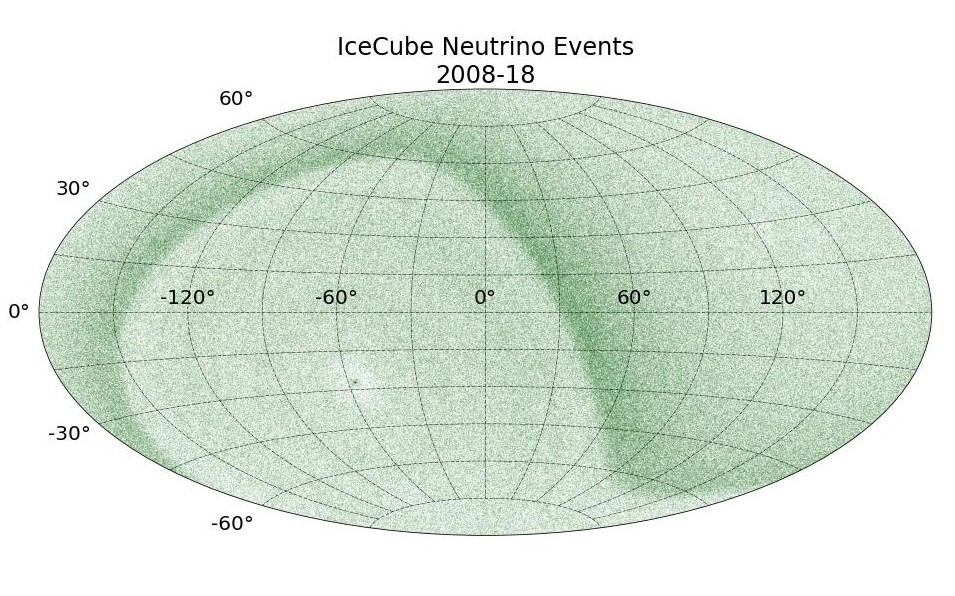
\includegraphics[width=0.6\columnwidth]{Images/nu-map.jpg}
	\end{center}
	\captionof{figure}{The darker regions indicate more density of events}
	\label{fig:nusky}	
\end{figure}
\subsection{\large Pulsars - ATNF}
The pulsar dataset used in this project is from ATNF catalogue version 1.68, which currently includes 3341 pulsars$^{~\cite{ATNF}}$. We only needed the right ascension and declination of each pulsar for this project.
\begin{figure}[!ht]
	\begin{center}
		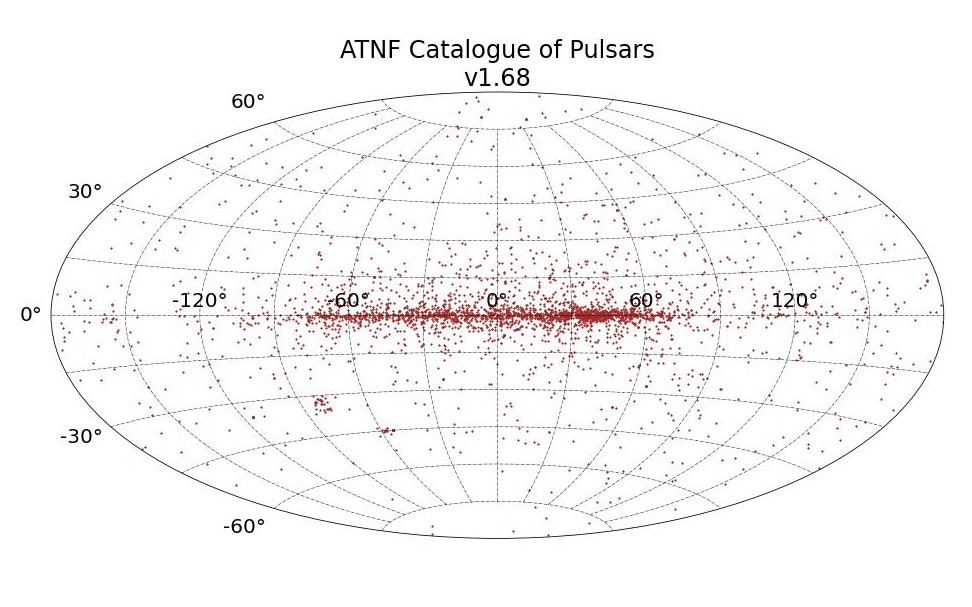
\includegraphics[width=0.6\columnwidth]{Images/pulsar-map.jpg}
	\end{center}
	\captionof{figure}{}
	\label{fig:psrsky}	
\end{figure}
\newpage
\section{\Large ANALYSIS}
\subsection{\large Pre-Processing}
We chose neutrino occurrences with declination within 5$^\circ$ of the pulsar for our research. The majority of pulsars are found near the galactic plane.
Because there are only two pulsars with > 85$^\circ$ (85.5$^\circ$ and 86.7$^\circ$), we included neutrinos within 5$^\circ$ of the poles for completeness.
%For this project, we only needed the RA and Declination of the pulsars.The angular reso

\subsection{\large Maximum Likelihood Estimation}
For this project, we used the unbinned maximum likelihood ratio estimation method as in ~\cite{Hooper,Kamionkowski,LuoZhang,Li22}.
For a dataset of $N$ events, if $n_s$ signal events are attributed to a pulsar, the probability
density of an individual event $i$ is given by:
\begin{equation}
	P_i = \frac{n_s}{N} S_i + (1-\frac{n_s}{N}) B_i,
	\label{eq:prob}
\end{equation}
where $S_i$ and $B_i$ represent the signal and background pdfs, respectively.\\

The likelihood function ($\mathcal{L}$) of the entire
dataset, obtained from the product of each individual PDF can be written as:

\begin{equation}
	\mathcal{L} (n_s) = \prod_{i=1}^N P_i,
\end{equation}
where $P_i$ is the same as in Eq.~\ref{eq:prob}.\\
 The signal PDF is given by:
\begin{equation}
S_i = \frac{1}{2\pi\sigma_i^2}e^{-(|\theta_i-\theta_s|)^2/2\sigma_i^2}
\label{eq:S}
\end{equation}
where $|\theta_i-\theta_s|$ is the angular distance between the  pulsar and the neutrino, whereas $\sigma_i$ is the angular uncertainty in the neutrino position, expressed in radians. 

The background PDF ($B_i$) is determined by the solid angle within  $\delta$ of $\pm 5^{\circ}$ around each pulsar ($\Omega_{\delta \pm 5^{\circ}}$):
\begin{equation}
B_i=\frac{1}{\Omega_{\delta \pm 5^{\circ}}}
\end{equation}
\subsection{\large Detection Statistic}

 The detection statistic (or the $Z$-score) used to ascertain the presence of a signal is given by:
\begin{equation}
TS (n_s) = 2 \log \frac{\mathcal{L} (n_s)}{\mathcal{L} (0)}
\label{eq:TS}
\end{equation}
This test-statistic is the log-likelihood ratio of two hypotheses: $H_1$: Of all the $N$ events, $n_s$ are produced by the interested source. \\
$H_0$: All the N events are background events.

The likelihood ratio in Eq.~\ref{eq:TS} will indicate how likely it is that some of the neutrino events can be attributed to the interested source %we are trying to test the association with the diffuse neutrino flux.\\

\subsection{\large Wilk's Theorem}
Under the assumption of Null hypothesis ($H_0$) being true:
When the sample size is very large, then the distribution of the test statistic $TS$ approaches a $\chi^2$ distribution$^{\cite{Wilks}}$.\\
%\subsection{Final Task}
The objective was to find $\hat{n_s}$ such that $TS$ is \emph{maximized}. If $\max{TS(\hat{n_s})}$ = 0, then the Null-Hypothesis is true, and the interested pulsar is not the source of the neutrinos observed in it's neighbourhood region of the sky.


\section{\Large RESULTS}
\subsection{\large Gaussian Fit}
For each pulsar, we calculated the test-statistic $TS$ and $n_s$ for which $TS$ is maximum.
The detection significance is then given by $\sqrt{TS}$. The $\sqrt{TS}$ histogram is fitted to a Gaussian distribution, with the amplitude set at the ratio of the number of sources to the total number of bins per unit X-axis and the mean and standard deviation permitted to vary. Each bin's inaccuracy is equal to the square root of the total number of occurrences$^{~\cite{Kamionkowski}}$.

\begin{figure}[htb]
	\begin{center}
		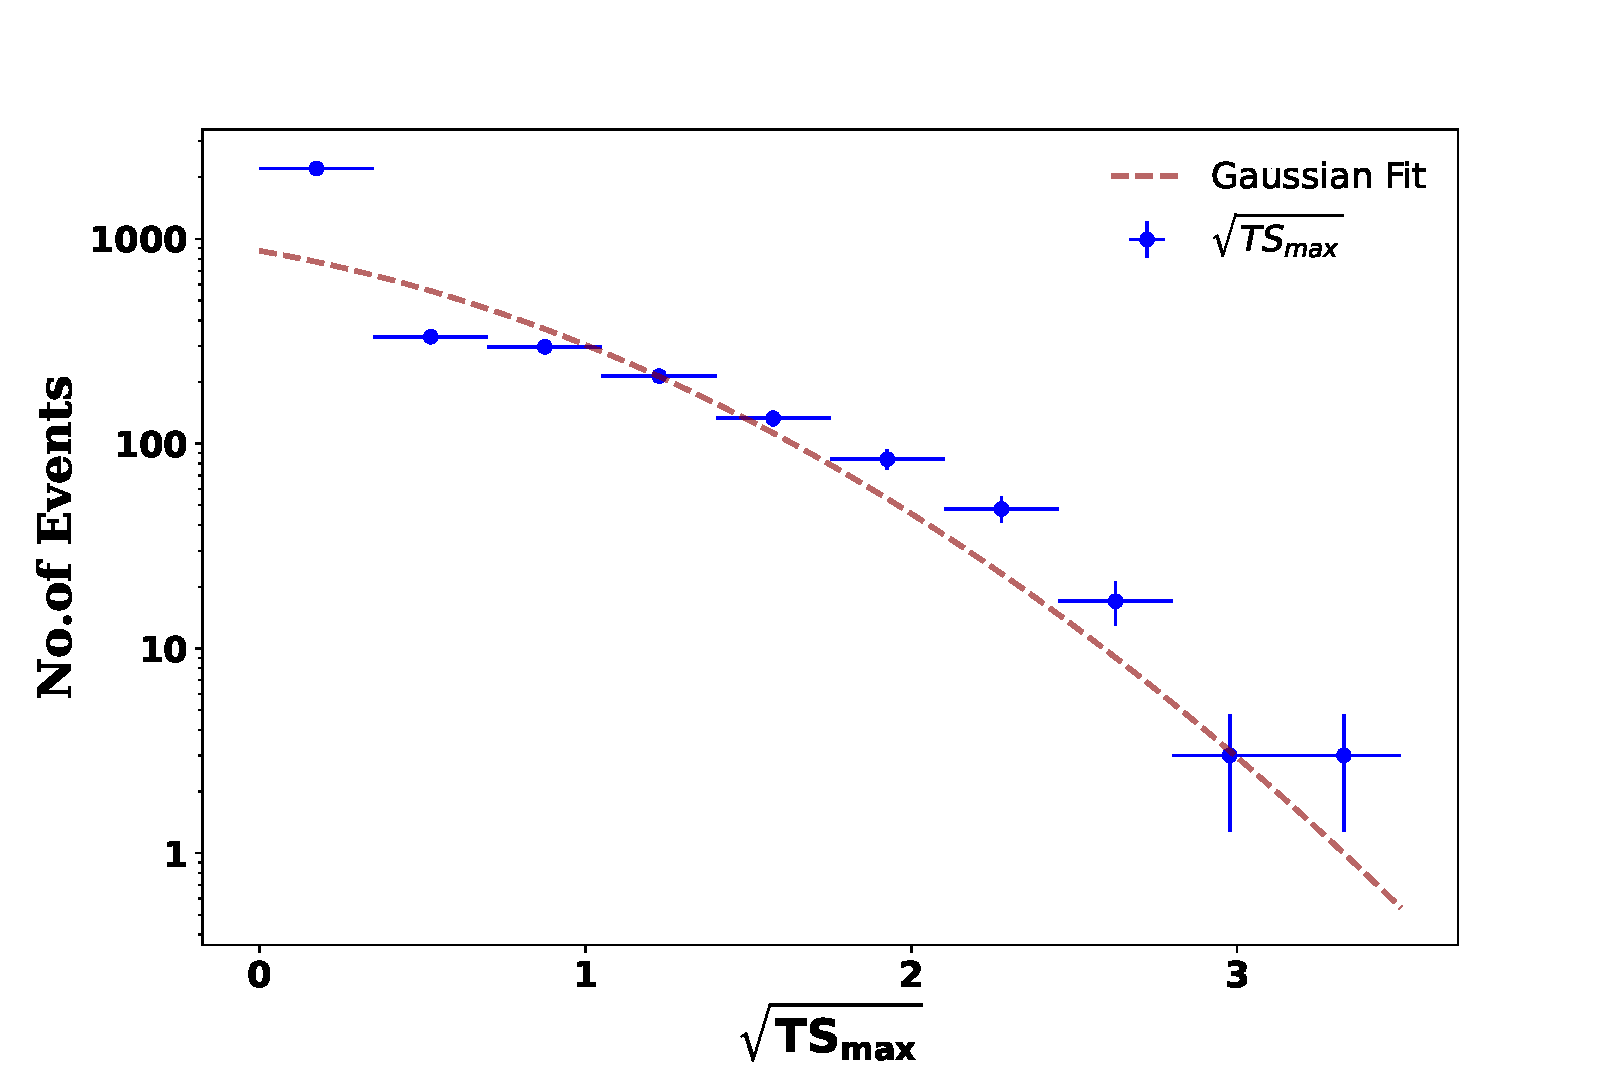
\includegraphics[width=0.75\columnwidth]{Images/sqrt(TSmax)final}
	\end{center}
	\captionof{figure}{Histogram of distributions of $\sqrt{TS_{max}}$ along with error bars given by square root of the number of events. The dashed
		red line shows the best Gaussian fit to this data.}
	\label{fig:gfit}	
\end{figure}

\subsection{\large Inferences}
From Fig.~\ref{fig:gfit} we can observe that the Gaussian distribution does not match the data well since there is a slight excess of events with very low $\sqrt{TS_{max}}$ values in the first bin. In contrast to the background, we do not see a statistically significant excess. Since $n_s$ is near to the physical boundary, the PDF of $TS(n_s)$ is a superposition of the $\chi^2$ and $\delta$ function, which may also contribute to this excess$^{~\cite{Wolf}}$.

The excess seen between 1.5 and 2.5 may be explained by errors in the PDF as well as by taking into account the trial factors$^{\cite{Hooper}}$. \\

\begin{table}[htb]
		\centering
		\large
		\setlength{\arrayrulewidth}{0.2mm}
		\setlength{\tabcolsep}{16pt}
		\begin{tabular}{P{2.25cm} P{1.5cm} P{1.5cm}}
			\hline\hline
			\centering
			Pulsar & \large $\tilde{n}_s$ & \large $TS_{max}(\tilde{n}_s)$\\
			\hline
			J1849+0037g & 43.5 & 12.3\\
			
			J1707-4341 & 17.4 & 11.8\\
			
			J1838-1849 & 16.5 & 10.4\\
			\hline\hline
		\end{tabular}
		\captionof{table}{Pulsars with highest $TS_{max}(\tilde{n}_s)$ values}
		\label{table1}
\end{table}
The distribution of occurrences with high significance as listed in (Table.~\ref{table1}) is consistent with background.Particularly the PSR B1509-58 which showed a 2.6$\sigma$ excess, when combined with the Super-Kamiokande and MACRO results$^{~\cite{Desai22}}$, has a $TS_{max}$ = 0.



%Skymap distribution of this statistic in galactic coordinates.

\begin{figure}[!ht]
	\begin{center}
		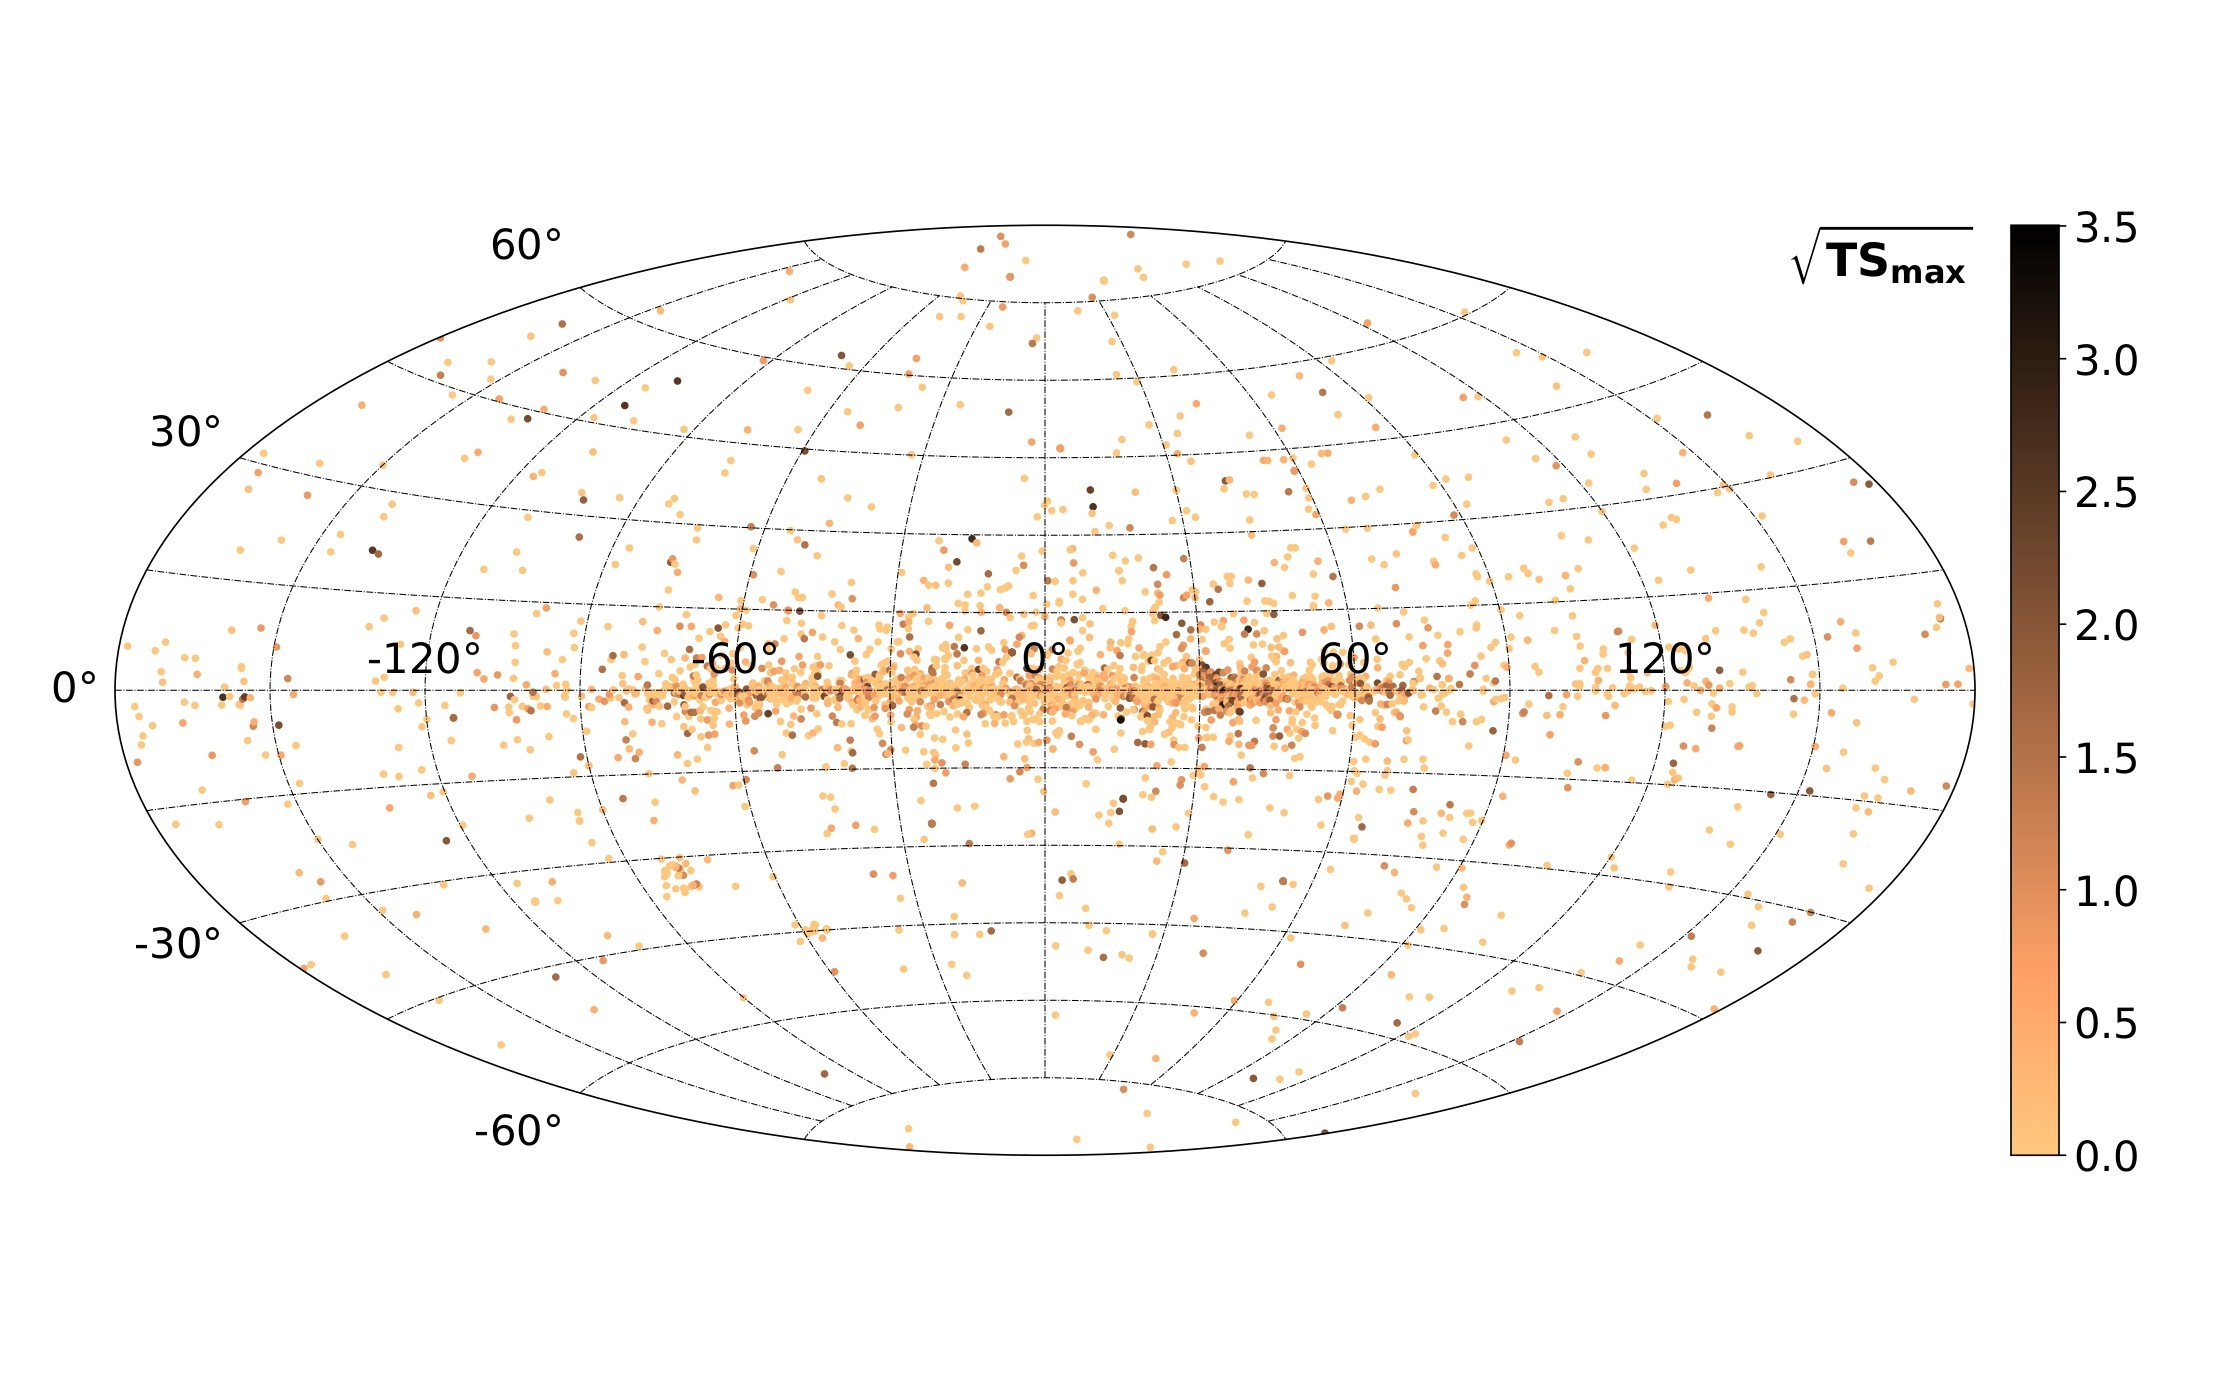
\includegraphics[width=0.7\columnwidth]{Images/psr-tsmax_hmp-HP-Galactic.jpg}
	\end{center}
	\captionof{figure}{Skymap distribution of$\sqrt{TS_{max}}$ in Galactic coordinates using Aitoff projection}
	\label{fig:skymap}	
\end{figure}

 As a result, we draw the conclusion that \emph{none} of the pulsars in the ATNF database at this time (on their own) are responsible for the diffuse neutrino flux seen by the IceCube.


\section{\Large SUMMARY/CONCLUSION}
In this work we look for a spatially significant correlation between individual radio pulsars and TeV energy neutrinos. For our analysis, we used the publicly available IceCube neutrino catalogue, comprising 11,34,450 neutrino events observed
%obtained from the muon track data using 
between 2008-2018, and all the 3341 radio pulsars compiled in the latest version of the ATNF catalog. The analysis was done using the unbinned maximum likelihood ratio method.
The distribution of the detection significance for each of the pulsars is shown in Fig. \ref{fig:gfit} and the skymap distribution in galactic coordinates in Fig.~\ref{fig:skymap}. A modest excess of events are seen in the first bin when the detection significance histogram is fitted to a Gaussian distribution. The occurences with high significance are consistent with the background. As a result, we can conclude that it is impossible for any of the known pulsars to be the source of the TeV-energy high energy neutrinos seen in IceCube.
%We then continue to perform a Monte Carlo test where a random pulsar RA, Dec are generated and is analysed against the neutrino database.
\newpage
\section*{\Large ACKNOWLEDGMENTS}
I thank the Dept. of Physics, IITH for giving me this wonderful oppurtunity to credit the project work we do.\\
I am extremely grateful to Prof. Shantanu Desai for guiding me through this entire project. %I am also thankful to the IceCube collaboration for making their point source neutrino catalog publicly available.
\section*{New things learnt}
\begin{enumerate}
	\item Learnt how neutrinos are produced and detected.
	\item Learnt about likelihoods, maximum likelihood estimations.
	\item Read various literature on IceCube, Neutrinos and likelihood analysis.
	\item Learnt to use Linux, terminal/command-line, Git-GitHub.
	\item Improved coding with python and learnt to apply various python libraries (numpy, numba, multiprocessing, etc) to parallelize the code execution and shorten the compile time.
\end{enumerate}
%\section*{}
In a future work, we will include a stacked contribution from all the pulsars
\newpage
%Bibliography
\bibliographystyle{unsrtnat}
\bibliography{template}

\end{document}
